\documentclass[11pt,a4paper]{article}
\usepackage{amsmath,amssymb,amsthm}
\usepackage{booktabs}
\usepackage{graphicx}
\usepackage{hyperref}
\usepackage[margin=2.5cm]{geometry}
\usepackage{enumitem}
\usepackage{microtype}
\usepackage{tikz}
\usetikzlibrary{shapes.geometric,arrows.meta,positioning,calc}

\newtheorem{theorem}{Theorem}
\newtheorem{lemma}{Lemma}
\newtheorem{corollary}{Corollary}
\newtheorem{proposition}{Proposition}
\newtheorem{definition}{Definition}
\newtheorem{remark}{Remark}
\newtheorem{observation}{Observation}
\newtheorem{assumption}{Assumption}

\title{The Vote-Left Equilibrium: A Deterministic Coordination
Strategy for the Faithful in Social Deduction Games}
\author{Vincent Knight}
\date{\today}

\begin{document}

% TODO BEFORE SUBMISSION: archive tex/src/deviation_sweep/deviation_gain_sweep.csv
% on Zenodo, then replace every reference to the "supplementary material" /
% "exact-rational evaluation sweep" / "deviation_gain_sweep.csv" /
% "tex/src/deviation_sweep/main.py" with the Zenodo DOI.
% Call sites to update:
%   1. Introduction, Contributions paragraph (first mention of the file).
%   2. Statement of Theorem 1 ("the exact-rational evaluation sweep distributed with").
%   3. Proof of Theorem 1: both "archived as deviation_gain_sweep.csv ..." and
%      the verification-script path "tex/src/deviation_sweep/main.py".
% Theorem 2 is now fully analytical and no longer references the CSV.

\maketitle

\begin{abstract}
\emph{The Traitors} is a social deduction game in which an informed minority
of Traitors face an uninformed majority of Faithful, and the recurring
question facing the Faithful is how to vote. Random voting is known to be
optimal for the uninformed majority under simultaneous-signal protocols
\cite{braverman2008}, but when votes are cast individually, random votes are
indistinguishable from strategic ones and the Faithful remain exposed to
coordinated Traitor collusion. We introduce the \emph{Vote-Left protocol}, a
deterministic rule under which every player votes for the next surviving
player in a fixed cyclic ordering. Under full compliance every surviving
player receives exactly one vote, so the banishment distribution coincides
with random voting; since prescribed votes are deterministic functions of
public information, any deviation is immediately identifiable. Combined with
a simple punishment rule, Vote-Left constitutes a Perfect Bayesian
Equilibrium for every state with \(n_t > 2m_t + 2\), a region that
contains every televised configuration. We characterise the Traitors'
best response in the late-game phase (\(n_t \leq 2m_t + 2\)): deviate
via collusion once the Faithful no longer have enough votes to guarantee
punishment. Across the configurations played on television, Vote-Left
raises the Faithful's winning probability by a factor of approximately
three over random voting under collusion.
\end{abstract}

\section{Introduction}

Social deduction games pit an informed minority against an uninformed
majority, and have become a popular setting for studying voting,
communication, and the use of public information under uncertainty. The
classical example is the Mafia game \cite{davidoff1986}, in which Mafia
members covertly eliminate citizens at night and, by day, the full group
votes to eliminate a suspect. \emph{The Traitors} (originally \emph{De
Verraders}, Netherlands, 2021) adapts this structure for television: a host
assigns a small group as Traitors (who know one another), the remainder
are Faithful, and play alternates between night murders and public
banishment votes until either all Traitors have been eliminated (Faithful
win) or the Traitors reach parity (Traitor win).

The natural baseline strategy for the Faithful is to vote at random.
Braverman, Etesami and Mossel \cite{braverman2008} showed that, under a
simultaneous-signal randomisation protocol, random voting is in fact
optimal for the citizens in Mafia without detectives, and Migda\l{}
\cite{migdal2010} subsequently derived a closed-form expression for the
winning probability under mutual random play. Wang \cite{wang2024} then
showed that when votes are cast individually the Traitors can substantially
improve their odds through coordinated collusion: an individual random
vote is indistinguishable from a strategic one, so a colluding Traitor
coalition is shielded by the same noise that protects the Faithful. The
Faithful are therefore caught in a tension between the optimality of random
voting in the abstract simultaneous-signal model and the vulnerability of
random voting in the actual game played on television.

We introduce the \emph{Vote-Left protocol} to resolve this tension. Every
player votes for the next surviving player in a fixed cyclic ordering, one
instance of a broader class of single-cycle derangements that share the
same properties. Under full compliance the protocol reproduces the uniform
expectation of random voting, so the day-phase distribution is unchanged; at
the same time, prescribed votes are deterministic functions of public
information, so any deviation from the protocol is immediately detectable.
Combined with a punishment rule, Vote-Left constitutes a Perfect Bayesian
Equilibrium (PBE) for every state with \(n_t > 2m_t + 2\), and we
characterise the Traitors' optimal deviation timing in the late-game phase.

\subsection*{Contributions and outline}

This paper makes four contributions. First, we introduce the Vote-Left
protocol and show that, combined with a punishment rule, it constitutes a
Perfect Bayesian Equilibrium for every state with \(n_t > 2m_t + 2\)
(Section~\ref{sec:equilibrium}). Second, we characterise the late-game
phase \(n_t \leq 2m_t + 2\) in which Traitor deviation becomes rational,
and define the optimal late-game strategy \(\sigma^\dagger\)
(Section~\ref{sec:timing}). Third, we show that Vote-Left raises the
Faithful's winning probability by a factor of approximately three relative
to random voting under collusion. Fourth, we release \texttt{backstab},
an open-source Python library that implements exact arithmetic for known
theoretical measures and a Monte Carlo engine to simulate seasons of
the show.

A typical season features $n \in \{20, \ldots, 25\}$ players with
$m \in \{3, 4\}$ Traitors. Across approximately 80 international seasons,
across approximately 30 countries,
the Traitors
Wiki\footnote{\url{https://thetraitors.fandom.com/wiki/List_of_Winners}}
records a 59\% Traitor win rate as shown in Figure~\ref{fig:outcomes_by_country}. 
Under mutual random play, which is known to be
optimal for the Faithful, the Migda\l{}
recurrence~\eqref{eq:migdal} gives a Traitor win rate $w(n, m)$ between
$0.624$ (at $n = 25$, $m = 3$, exactly $2{,}110{,}959/3{,}380{,}195$) and
$0.864$ (at $n = 22$, $m = 4$, exactly $311{,}471/360{,}448$) across the
televised configurations. The gap between the empirical 58\% and the
predicted 62--86\% plausibly reflects partial information from social
discussion, yet the Traitor advantage clearly persists. Vote-Left removes
the vote-manipulation channel while leaving the rest of the social
dynamics of the show intact.

\begin{figure*}[htbp!]
    \begin{center}
        
\includegraphics[width=\textwidth]{fig_tv_outcomes.pdf}
        \caption{\textbf{The outcomes by country}
        More than 80 seasons of the show have been played. The overall win rate
        shows a clear advantage to the traitors.
        }
        \label{fig:outcomes_by_country}
    \end{center}
\end{figure*}

\section{Model}\label{sec:model}

We define the Traitors Game \(\mathrm{TG}(n,m)\) as
follows. A set of \(n\) players is arranged in a fixed cyclic ordering. A
subset of \(m\) of them are Traitors; the remaining \(n - m\) are Faithful.
The Traitors know one another, while the Faithful know only their own role.
Play alternates between a day phase (a public vote, with the most-voted
player banished, ties broken uniformly at random, and the banished player's
role revealed) and a night phase (the Traitors murder one Faithful). The
Faithful win when all Traitors have been banished; the Traitors win as soon
as parity is reached (\(|T| \geq |F|\)). We suppress elements of the television
show such missions, shields, and
recruitment and the end game, all of which are discussed briefly in
Section~\ref{sec:discussion}.
Figure~\ref{fig:game} summarises the game structure and contrasts random
voting with Vote-Left. 


\begin{figure*}[htbp!]
    \begin{center}
        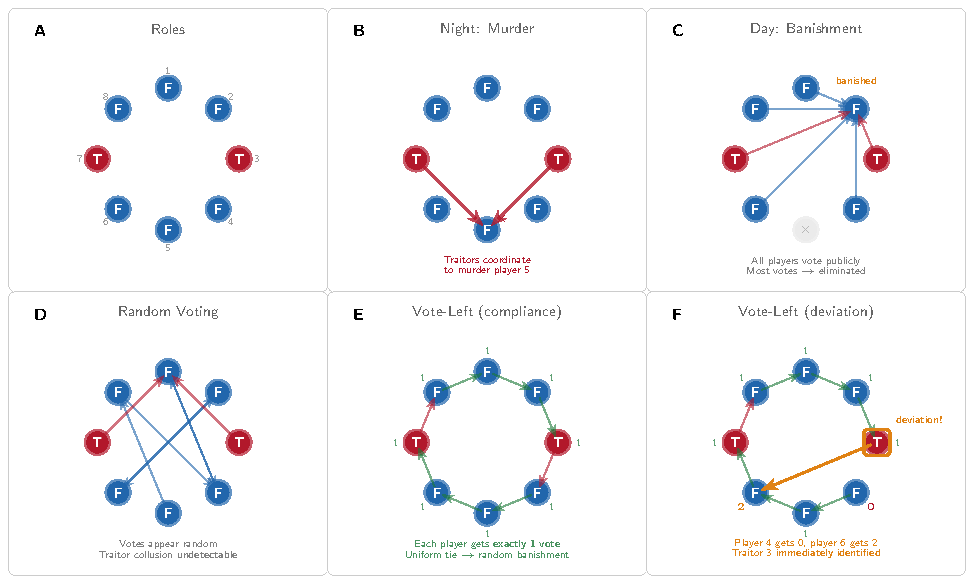
\includegraphics[width=\textwidth]{panel_diagram.pdf}
        \caption{\textbf{The Traitors game and voting strategies.}
        \textbf{A,} Eight players (F for Faithful in blue, T for Traitor in red)
        arranged in a circle with two Traitors. \textbf{B,} Night phase: the
        Traitors coordinate to murder a Faithful (player 5).
        \textbf{C,} Day phase: the public vote leads to banishment.
        \textbf{D,} Under random voting, Traitor collusion (the two
        red arrows converging on player 1) is indistinguishable from
        random noise. \textbf{E,} Under Vote-Left, each player votes
        for the next in the cycle, and every player receives exactly
        one vote. \textbf{F,} A Traitor who deviates from Vote-Left
        breaks the uniform count (player 4 receives 0, player 6
        receives 2), making the deviation immediately identifiable.}
        \label{fig:game}
    \end{center}
\end{figure*}

\begin{assumption}[Individual maximisation]
All players maximise their individual winning probability.
\end{assumption}

\begin{remark}[Win condition and tie-breaking]\label{rem:boundary}
We use the parity win condition (\(|T| \geq |F|\), i.e.\ \(m \geq \lceil n/2
\rceil\)), appropriate for \emph{The Traitors}' rules.  Migda\l{}
\cite{migdal2010} uses the strict-majority condition (\(m > n - m\)); the two
agree for odd \(n\) and differ only at exact ties for even \(n\).  We assume uniform
random tie-breaking; in practice, the show uses a revote followed by a random
draw.
\end{remark}

A \textbf{strategy} for player \(i\) maps observable game history to a
distribution over surviving players (excluding themself). We write \(L(i)\) for
the next surviving player after~\(i\) in the cyclic ordering.

\subsection{Baseline winning probability}

The following recurrence, due to Migda\l{}~\cite{migdal2010}, gives the
exact Traitor win probability under mutual random play. We restate it here
for completeness, using the parity win condition of
Remark~\ref{rem:boundary}, and provide a short proof for the reader's
convenience.

\begin{proposition}[Migda\l{} recurrence, adapted]\label{prop:migdal}
Let \(w(n,m)\) denote the Traitor win probability under mutual random play from
state \((n,m)\).  Then
\begin{equation}\label{eq:migdal}
w(n,m) = \begin{cases}
  0 & \text{if } m = 0, \\
  1 & \text{if } m \geq \lceil n/2 \rceil, \\[4pt]
  \dfrac{n-m}{n}\,w(n-2,m) \;+\; \dfrac{m}{n}\,w(n-2,m-1) & \text{otherwise.}
\end{cases}
\end{equation}
\end{proposition}

\begin{proof}[Proof (following Migda\l{}~\cite{migdal2010})]
The boundary cases follow directly from the win conditions.  For interior
states, one full round consists of a day phase followed by a night phase.

\textit{Day phase.}  Under mutual random play each surviving player is equally
likely to be banished.  With probability \(m/n\) the banished player is a Traitor,
    reducing the state to \((n-1, m-1)\) (Figure~\ref{fig:migdal_recursion} - B); with probability \((n-m)/n\) it is a
Faithful, reducing the state to \((n-1, m)\) (Figure~\ref{fig:migdal_recursion} - D).

\textit{Night phase.}  The Traitors murder one Faithful, decreasing \(n\) by a
further one while leaving \(m\) unchanged.  After both phases the state is
\((n-2, m-1)\) (Figure~\ref{fig:migdal_recursion} - C) or \((n-2, m)\) (Figure~\ref{fig:migdal_recursion} - E), respectively.

Applying the Markov property and taking expectations gives~\eqref{eq:migdal}.
The recurrence terminates because \(n\) decreases by two each round and the
boundary is eventually reached.
\end{proof}

\begin{figure}[htbp!]
\centering
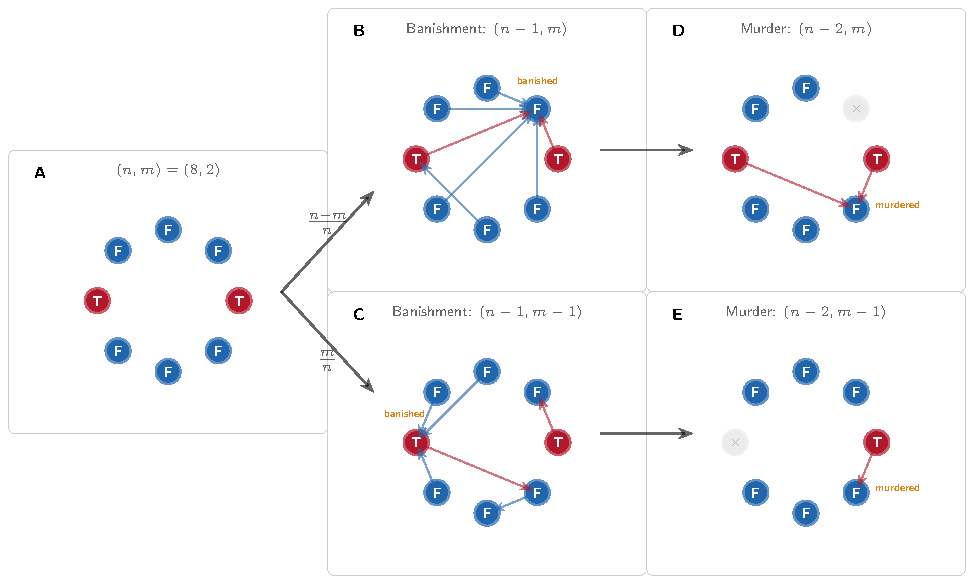
\includegraphics[width=\textwidth]{migdal_recursion.pdf}
    \caption{\textbf{Recursion relationship for \(w(n, m)\).}
        \textbf{A,} Initial state for \(w(8, 2)\), given random voting the
        next step could either be \textbf{B,} or \textbf{D}. 
        This leads immediately to \textbf{C,} or \textbf{E} respectively.}
\label{fig:migdal_recursion}
\end{figure}


\section{The Vote-Left Protocol}

\begin{definition}[Cyclic voting protocol]
    A \emph{cyclic voting protocol} prescribes that each player votes for a
    target determined by a \textbf{shared} fixed single-cycle permutation of the
    surviving players. The \emph{Vote-Left protocol} is the instance where each
    player votes for \(L(i)\).
\end{definition}

\begin{observation}[Uniform marginal and observability]\label{obs:main}

Under full compliance: (i)~every player receives exactly one vote, producing a
uniform \(1/n_t\) banishment probability, identical to random voting; (ii)~any
deviation is immediately and publicly identifiable, since prescribed votes are
deterministic functions of public information.

\end{observation}

Random voting achieves (i) but not (ii): a Traitor who concentrates their
vote is indistinguishable from a citizen who happened to draw that target
at random. Vote-Left achieves both properties simultaneously.

\section{Equilibrium Analysis}\label{sec:equilibrium}

\subsection{Strategy profile}

\begin{definition}[Vote-Left with Punishment]\label{def:equil}

Vote-Left with Punishment is the strategy profile \(\sigma^*\), governed by a
public state \(s \in \{\mathtt{comply},\, \mathtt{punish}(j)\}\) common to all
players:
\begin{itemize}[leftmargin=1.4em,itemsep=1pt,topsep=2pt]
    \item In state \(\mathtt{comply}\), every surviving player \(i\) votes for
  \(L(i)\). If a deviation is observed on the vote, the state transitions to
  \(\mathtt{punish}(j)\), where \(j\) is the deviator. In the rare event that
  two or more players deviate in the same round, \(j\) is taken to be the
  deviator with the smallest index in the fixed cyclic ordering, and any
  remaining deviators are punished in subsequent rounds using the same rule.
\item In state \(\mathtt{punish}(j)\), every surviving player votes for
  \(j\); after \(j\)'s banishment, the state returns to \(\mathtt{comply}\).
\end{itemize}
Traitors play Vote-Left in \(\mathtt{comply}\) and murder a uniformly random
Faithful at night.
\end{definition}


\subsection{Deviation payoff analysis}

We compare the Traitors' exact expected payoffs under compliance and under
deviation from a state \((n_t, m_t)\). Let \(w(n, m)\) denote the Traitor
win probability under the Migda\l{} recurrence \cite{migdal2010}.

\textbf{Compliance value.} Under \(\sigma^*\), every surviving player
votes cyclically, so each round reduces the state by exactly one of the
two pairs considered in Proposition~\ref{prop:migdal}. The continuation
value under compliance therefore equals the random-play value,
\(V_{\mathrm{comply}}(n_t, m_t) = w(n_t, m_t)\). This is the quantity
that any deviation must be compared against.

\begin{lemma}[No profitable deviation for a Faithful]\label{lemma:faithful}
Under \(\sigma^*\), if a Faithful player \(i\) deviates from Vote-Left, 
their individual winning probability becomes 0.
\end{lemma}

\begin{proof}
If \(i\) deviates, the deviation is publicly observable (since votes are
deterministic under compliance). The state transitions to
\(\mathtt{punish}(i)\), and in the next day phase, all players vote for
\(i\), so \(i\) is banished with probability 1. A banished player cannot
win, so \(i\)'s individual winning probability is 0. Under compliance, \(i\)
is not banished in this round, so their winning probability is strictly
positive. Thus, deviation is irrational.
\end{proof}

\begin{lemma}[No profitable deviation for a Traitor]\label{lemma:traitor}
Under \(\sigma^*\), if a Traitor player \(i\) deviation from Vote-Left in a state
with \(n > 2m + 2\) implies that their individual winning probability becomes 0.
\end{lemma}

\begin{proof}
If \(i\) deviates, the deviation is publicly observable. The state transitions
    to \(\mathtt{punish}(i)\) with \(n - 1\) players and \(m\) Traitors.
    The night phase leads to \(n - 2\) players and \(m\) Traitors.
    This leads to the next day phase with \(n - 2 - m\) Faithful. They can punish the
    \(i\) if and only if \(n - 2 - m > m \Leftrightarrow n > 2m +2\).
    If this condition does not hold then all players vote for \(i\), so \(i\) is
banished with probability 1. A banished player cannot win, so \(i\)'s
individual winning probability is 0. Under compliance, \(i\) is not banished
in this round, so their winning probability is strictly positive. Thus,
deviation is irrational.
\end{proof}

\begin{theorem}[Perfect Bayesian Equilibrium]\label{thm:pbe}
\(\sigma^*\) constitutes a PBE of \(\mathrm{TG}(n, m)\) for every state with
\(n > 2m + 2\).
\end{theorem}

\begin{proof}
Sequential rationality follows from Lemmas~\ref{lemma:faithful}
and~\ref{lemma:traitor}: no player can profitably deviate given the prescribed
strategies.
\end{proof}

\section{Traitor deviation timing}\label{sec:timing}

The equilibrium of Section~\ref{sec:equilibrium} characterises rational
behaviour in every state satisfying \(n_t > 2m_t + 2\). In the
complementary \emph{late-game phase}, \(n_t \leq 2m_t + 2\), the Faithful
no longer have enough members to guarantee punishment after a night murder,
and Lemma~\ref{lemma:traitor} no longer applies.

\textbf{Late-game structure.} When \(n_t \leq 2m_t + 2\), a Traitor who
deviates is detected and placed in state \(\mathtt{punish}(i)\). After the
following night murder there are at most \(n_t - 2 - m_t \leq m_t\)
Faithful remaining. The Faithful can no longer outvote the Traitors in the
punishment round, so the punishment threat ceases to be credible and
deviation becomes individually rational.

\textbf{Optimal late-game strategy.} We define \(\sigma^\dagger\) as the
strategy that complies with Vote-Left whenever \(n_t > 2m_t + 2\) and
deviates via full collusion when \(n_t \leq 2m_t + 2\). This is
implemented as \texttt{OptimalTimingDeviation} in \texttt{backstab}. For
the televised range \(m_t \in \{2, 3, 4\}\) the late-game threshold is
\(n_t \leq 6\), \(8\), or \(10\) respectively, corresponding to one to
three rounds near the end of a typical season. We assess the empirical
effect of \(\sigma^\dagger\) in Section~\ref{sec:sim}.

\section{Numerical evaluation}\label{sec:sim}

In this section we bring the exact analysis of
Sections~\ref{sec:equilibrium} and~\ref{sec:timing} together with Monte
Carlo simulation, in order to assess robustness across game sizes and to
quantify how Vote-Left changes the Faithful's winning probability. All
simulations were run using the \texttt{backstab} library. The simulation
loop is shown in Figure~\ref{fig:simulation}; compliance outcomes match
the exact \(w(n, m)\) values to within Monte Carlo error.

\begin{figure}[htbp!]
\centering
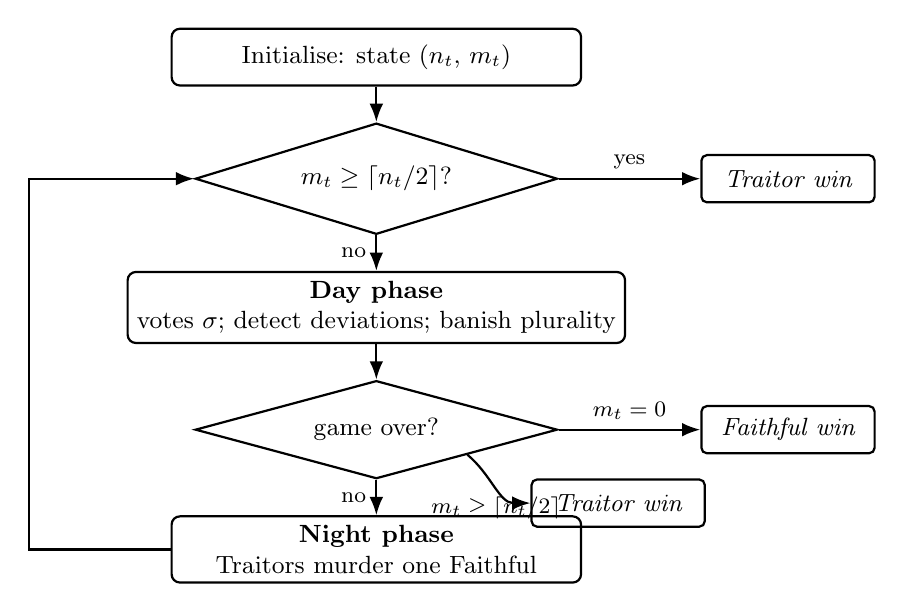
\begin{tikzpicture}[
  node distance=0.5cm,
  box/.style={
    rectangle, rounded corners=3pt, draw, thick,
    minimum width=5.2cm, minimum height=0.72cm,
    align=center, font=\small},
  dec/.style={
    diamond, draw, thick, aspect=2.5,
    minimum width=4.6cm, align=center, font=\small},
  res/.style={
    rectangle, draw, thick, rounded corners=2pt,
    minimum width=2.2cm, minimum height=0.60cm,
    align=center, font=\small\itshape},
  arr/.style={-Latex, thick},
]
  \node[box]  (init)
      {Initialise: state \((n_t,\,m_t)\)};
  \node[dec,  below=0.45cm of init]   (w1)
      {\(m_t \geq \lceil n_t/2 \rceil\)?};
  \node[box,  below=0.45cm of w1]     (day)
      {\textbf{Day phase}\\
       votes \(\sigma\); detect deviations;
       banish plurality};
  \node[dec,  below=0.45cm of day]    (w2)   {game over?};
  \node[box,  below=0.45cm of w2]     (night)
      {\textbf{Night phase}\\
       Traitors murder one Faithful};
  \node[res,  right=1.8cm of w1]  (Tw)   {Traitor win};
  \node[res,  right=1.8cm of w2]  (Fw)   {Faithful win};
  \node[res,  below right=0.3cm and 0.8cm of w2]  (Tw2)  {Traitor win};

  \draw[arr] (init) -- (w1);
  \draw[arr] (w1)   -- node[left,  font=\footnotesize]{no}  (day);
  \draw[arr] (w1)   -- node[above, font=\footnotesize]{yes} (Tw);
  \draw[arr] (day)  -- (w2);
  \draw[arr] (w2)   -- node[left,  font=\footnotesize]{no}  (night);
  \draw[arr] (w2.east) to[out=0, in=180]
      node[above, font=\footnotesize]{\(m_t = 0\)}  (Fw.west);
  \draw[arr] (w2.south east) to[out=-40, in=180]
      node[below, font=\footnotesize]
      {\(m_t \geq \lceil n_t/2 \rceil\)}            (Tw2.west);
  \draw[arr] (night.west) -- ++(-1.8, 0) |- (w1.west);
\end{tikzpicture}
\caption{\textbf{Monte Carlo simulation loop in \texttt{backstab}.}
One pass of the inner loop simulates a single game of
\(\mathrm{TG}(n, m)\). Win conditions are checked before the day phase
and again after the day-phase banishment; the night phase follows
whenever neither condition is met. The outer loop repeats for
\(N_{\mathrm{sims}}\) independent games and aggregates outcomes into
win rates and confidence intervals.}
\label{fig:simulation}
\end{figure}

\begin{figure}[hbtp!]
\centering
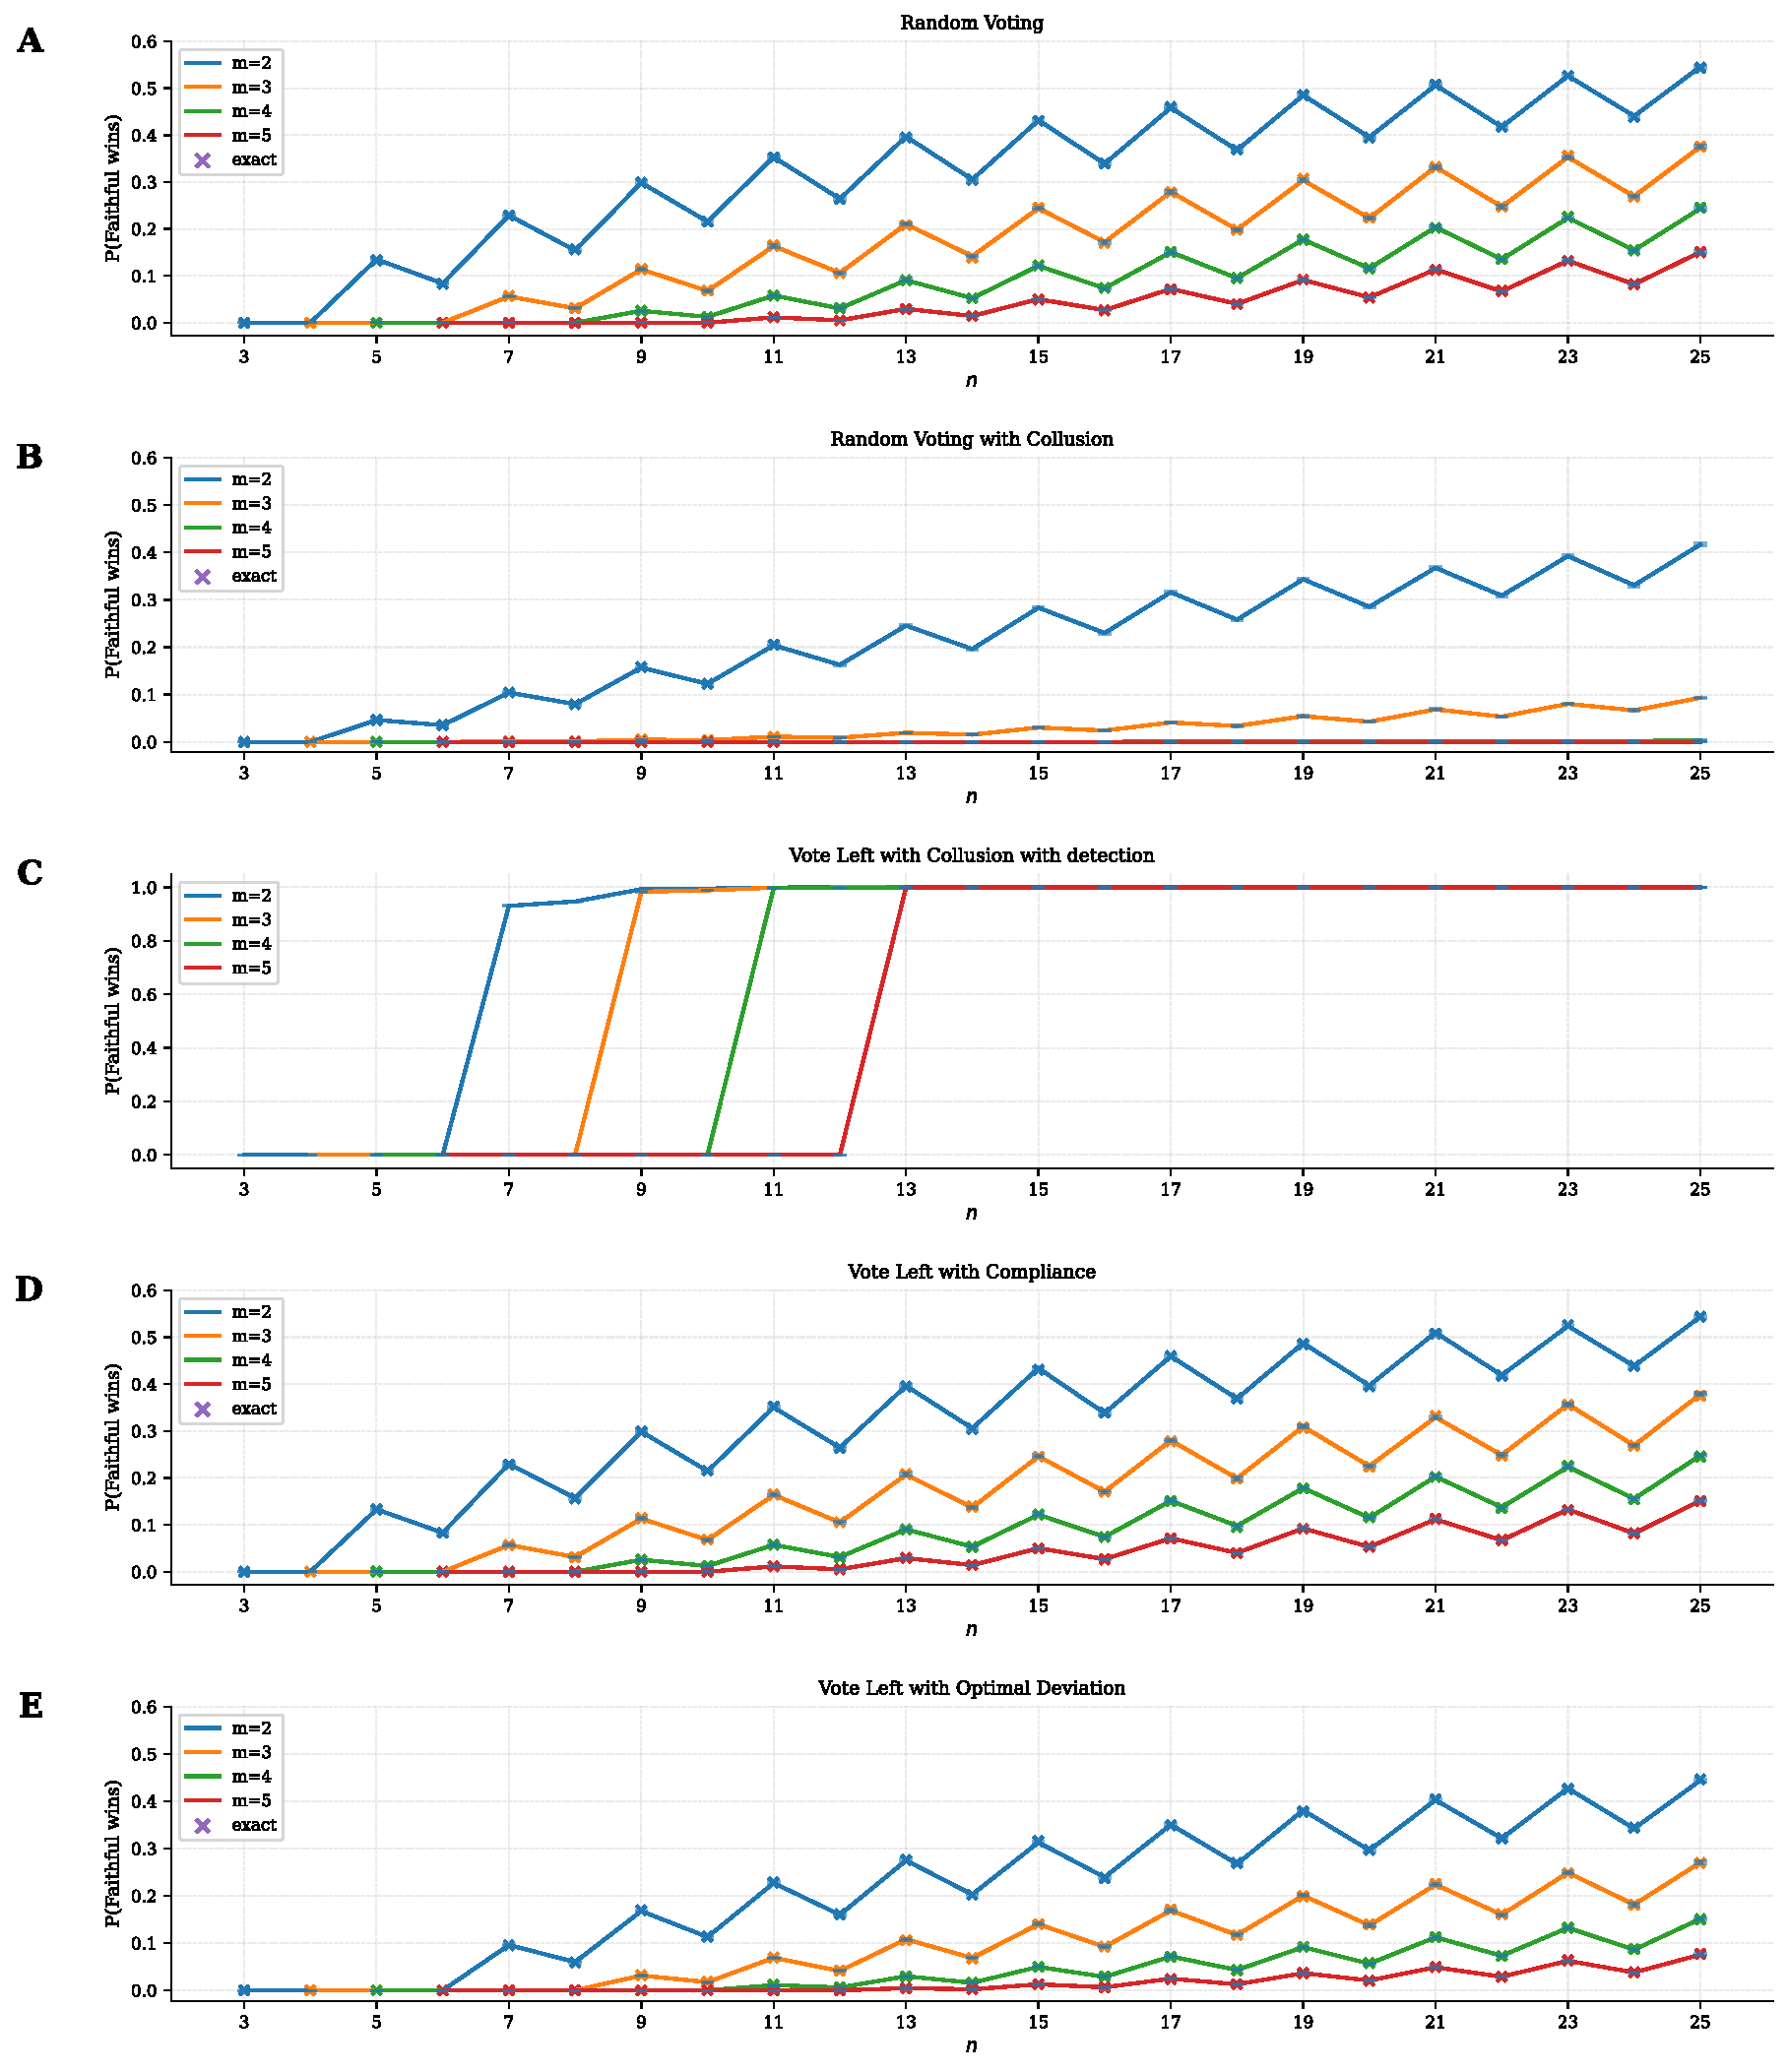
\includegraphics[width=\textwidth]{fig_strategy_comparison.pdf}
\caption{\textbf{Strategy comparison.} \textbf{A,} Faithful win rate
under four strategy profiles for \(\mathrm{TG}(22, 3)\), with 95\%
confidence intervals over 15{,}000 simulations per bar. The dashed line
is the exact value \(1 - w(22, 3) \approx 0.248\). RV and VL yield
identical compliance outcomes; collusion under RV (RV+C) collapses the
Faithful win rate to approximately 0.05, while Vote-Left with optimal
Traitor deviation (\(\sigma^\dagger\), VL+Opt) still yields a Faithful
win rate above 0.16. \textbf{B,} Faithful win rate under RV+C (orange)
and VL+Opt (blue) across all televised game configurations. Vote-Left
raises the Faithful win rate by a factor of approximately three or more
in every configuration.}
\label{fig:strategy}
\end{figure}

Figure~\ref{fig:strategy}A confirms that VL and RV produce identical
compliance outcomes, both near \(0.25\) and matching the exact value of
\(0.248\). Collusion under RV reduces the Faithful win rate to
approximately \(0.06\), whereas deviation under VL raises it
monotonically. Notably, even a constant deviation rate of \(p = 0.1\)
already more than doubles the Faithful win rate
(Figure~\ref{fig:strategy}B).

\begin{table}[htbp!]
\centering
\caption{Probability of a Traitor win across game configurations
(15{,}000 simulations per cell; standard error \(\leq 0.004\), so the
third decimal lies near the noise floor and should not be
over-interpreted). \textbf{Exact} gives \(w(n, m)\) from the Migda\l{}
recurrence; \textbf{RV} verifies this by simulation. \textbf{RV+C} is
random voting against Traitor collusion. \textbf{VL+Opt} is Vote-Left
against the optimal Traitor strategy \(\sigma^\dagger\). Lower values
are better for the Faithful.}
\label{tab:paramsweep}
\smallskip
\begin{tabular}{@{}ccccc@{}}
\toprule
\((n, m)\) & Exact & RV & RV+C & VL+Opt \\
\midrule
(15, 2) & 0.570 & 0.568 & 0.721 & 0.681 \\
(20, 3) & 0.776 & 0.777 & 0.956 & 0.864 \\
(22, 3) & 0.752 & 0.754 & 0.947 & 0.839 \\
(24, 3) & 0.731 & 0.736 & 0.936 & 0.816 \\
(25, 3) & 0.625 & 0.623 & 0.907 & 0.731 \\
(22, 4) & 0.864 & 0.860 & 0.998 & 0.929 \\
(25, 4) & 0.754 & 0.752 & 0.997 & 0.845 \\
\bottomrule
\end{tabular}
\end{table}

Table~\ref{tab:paramsweep} reports Traitor win probabilities at seven
configurations spanning the televised range of \emph{The Traitors}.
Two features stand out. First, the collusion penalty
(\textbf{RV} \(\to\) \textbf{RV+C}) is severe: the Traitor win rate
rises sharply across configurations and exceeds \(0.99\) in both
\(m = 4\) configurations, leaving the Faithful with virtually no
chance. Second, Vote-Left with optimal Traitor deviation
(\textbf{VL+Opt}) holds the Traitor win rate strictly below the
collusion baseline in every configuration; equivalently, it restores
the Faithful's winning probability by a factor of approximately three
at \((n, m) \in \{(22, 3), (20, 3)\}\) and by a factor of \(40\) or
more when \(m = 4\), where the collusion baseline is close to one.

\section{Discussion}\label{sec:discussion}

Our analysis covers the core Traitors game: a fixed roster of players, a
sequence of day votes and night murders, and a parity win condition for
the Traitors. Televised and parlour-game variants add further structure
that our model abstracts over. We discuss three natural extensions in
turn.

When the Traitors recruit a Faithful player mid-game, the recruited
player joins the Traitor coalition with full knowledge of Traitor
identities. The post-recruitment state is \((n_t, m_t + 1)\), and
compliance with Vote-Left remains rational for the recruited player
\emph{provided that the new state still satisfies the hypothesis of
Theorem~\ref{thm:pbe}}, that is, provided \(n_t > 2(m_t + 1) + 2\). Recruitment that fires early
(while \(n_t\) is large) lies comfortably within this bound; late
recruitment, near the endgame, can push the post-recruitment state into
the profitable-deviation region, in which case the recruit's incentives
align with late-game deviation (\(\sigma^\dagger\)) rather than with
compliance. Recruitment timing can also affect adjacency in the cyclic
ordering, and so it affects which Faithful the Traitors are best placed
to target once the late-game threshold is reached. A cleaner
characterisation of this recruitment-timing game is a natural extension
of our analysis.

If only a fraction \(q\) of the Faithful follow Vote-Left, the
non-compliant votes provide noise that can mask genuine Traitor
deviations, since a deviating Traitor now hides among the non-compliers
rather than standing out as the unique off-protocol vote. The critical
value of \(q\) below which the Faithful can no longer reliably attribute
deviations to Traitors will depend on the noise model and on the group
size. Characterising this threshold, and the resulting minimax
trade-off against random voting, is a natural open problem.

The televised format of \emph{The Traitors} includes a final end-game
round, typically with three to five players remaining, in which the
Faithful must vote unanimously to expel all remaining Traitors in order
to win; if any Traitor survives, the Traitors share the prize regardless
of relative numbers. This end-game mechanism replaces the parity win
condition and lies outside our model. A formal treatment, in which the
Faithful face a commitment and coordination problem under incomplete
information in a single climactic vote, is a natural extension of the
analysis.

The optimal late-game strategy \(\sigma^\dagger\) switches cleanly
between compliance and full collusion at the threshold \(n_t = 2m_t + 2\),
but it is not the only candidate worth studying. Mixed strategies that
deviate with some probability \(p < 1\) at every state, and gradual
strategies that increase the deviation probability as the game
progresses, both create detection exposure during the main game and can
in principle balance the punishment cost against the cumulative
concentration benefit. A systematic characterisation of the profitable
region in the joint (timing, intensity) space, and of how it shifts
with the cyclic ordering and recruitment, is a natural extension of our
analysis.

\section{Conclusion}

Vote-Left is a deterministic cyclic voting rule that reproduces the
uniform marginal of random voting while making any deviation observable.
It constitutes a PBE for every state with \(n_t > 2m_t + 2\)
(Theorem~\ref{thm:pbe}), and raises the Faithful's winning probability
by a factor of approximately three over random voting under collusion
across the configurations played on television.

The Traitors' best response is to comply throughout the main game and
deviate via collusion in the late-game phase (\(n_t \leq 2m_t + 2\)),
gaining approximately 6 to 11 percentage points over the compliance
baseline. The boundary is sharp: the punishment mechanism is credible
throughout the main game and ceases to be so only in the final rounds.

Operationally, Vote-Left is simple over the main game: each player
votes for the next surviving player in the agreed cyclic ordering. The
robustness of the protocol depends on the Faithful retaining a strict
majority through the main game, so that the punishment of a detected
deviator is credible; this is exactly the region of
Theorem~\ref{thm:pbe}. Whether human players would actually adopt a
deterministic protocol over the in-room deliberation that television
formats encourage is an empirical question, and one that we hope to
explore in future work.

\bibliographystyle{plain}
\bibliography{refs}

\end{document}
